\documentclass[12p]{article}
\usepackage{a4wide} %strona formatu a4, szeroko wypełniona tekstem
\usepackage{amsmath} %dodatkowe komendy, np. \underset
\usepackage{polski} %polskie litery
\usepackage{graphicx} 
\linespread{1.3}
\usepackage{geometry} 
\newgeometry{tmargin=3cm, bmargin=3cm, lmargin=4.0cm, rmargin=2.5cm}


\begin{document}

\tableofcontents
\newpage
\quad Celem pracy jest przedstawienie algorytmów kryptograficznych oraz możliwych ataków. Następnie implementacja 2 algorytmów na systemie wbudowanym oraz porównanie ich wydajności w zależności od rozmiaru szyfrowanych danych.
\newline
\newline
!!!!!!!!!!!!! będzie więcej opisu !!!!!!!!!!!!!!!!

\newpage
\section{Kryptografia}
%-----------------------------------
%	Rozdział 1
%-----------------------------------
\subsection{Wprowadzenie}

\quad W obecnych czasach dużym zainteresowaniem cieszy się bezpieczeństwo cybernetyczne, którego szczególną częścią jest kryptografia. Szczególnie ważne zastosowanie znajduje w branży informatycznych, militarnej, urzędach, grupach developerskich czy bankowości. Kryptografia pojawiła się znaczniej wcześniej niż platformy obliczeniowe, zainteresowali się nią już ludzie z czasów starożytnych, pojawiła się wraz z umiejętnością pisania. Powodem istnienia kryptografii jest bezpieczne i prywatne dostarczanie wiadomości. Znajduje szczególne zastosowanie w przypadku danych przesyłanych drogą internetową, dzięki kryptografii możliwe jest zapewnienie bezpieczeństwa cybernetycznego przesyłanych danych. W zależności od stopnia poufności informacji, którą chcemy zaszyfrować, aby niepożądane osoby jej nie odczytały można zastosować odmiennych algorytmów szyfrowania. 

\quad Kryptologia to połączenie kryptografii i kryptoanalizy. W języku greckim 'kryptos' oznacza ukryty, zaś 'logos' tłumaczone jest jako słowo. Kryptologia jest dziedziną zajmującą się ukrywaniem tekstu jawnego. Kryptografia jest dziedziną węższą od kryptologii, jest badaniem technik matematycznych związanych z bezpieczeństwem informacji. Do bezpieczeństwa danych można zaliczyć poufność informacji, uwierzytelnienie użytkowników i pochodzenia danych, a także integralność danych. Słowo kryptologia składa się z dwóch greckich słów: 'kryptos' znaczący ukryty i 'graph' oznaczający pisanie, jest to nauka o zabezpieczaniu danych. Za pomocą technik kryptograficznych możliwe jest zaszyfrowanie jawnego tekstu, w taki sposób aby niepożądana osoba nie mogła ich odczytać. Drugą gałęzią kryptologii jest kryptoanaliza, która zajmuje się analizą i możliwymi sposobami odszyfrowania kodu kryptograficznego.

\subsection{Powszechne ataki}
\quad W większości metod tunelowania wykorzystano szyfrowanie, które można podzielić na symetryczne i asymetryczne. Proces szyfrowania polega na przekształceniu tekstu jawnego w tekst zaszyfrowany. Szyfrowanie asymetryczne odbywa się przy użyciu dwóch kluczy: publicznego i prywatnego. Klucz publiczny jest wykorzystywany do szyfrowania danych, zaś klucz prywatny do ich odszyfrowywania. W przypadku szyfrowania symetrycznego wykorzystywany jest jeden klucz, co prowadzi do mniejszego bezpieczeństwa szyfrowania kosztem szybszego procesu szyfrowania i odszyfrowywania danych. 
Długość klucza określana jest w bitach. Dla klucza o mniejszej długości proces szyfrowania i odszyfrowywania przebiega szybciej. Wadą jest mniejsze bezpieczeństwo przesyłanych danych. Powszechnie w przypadku szyfrowania asymetrycznego nie stosuje się kluczy krótszych niż 4096 bitów. VPN umożliwia uwierzytelnienie urządzenia, sprawdzenie integralności pakietów i szyfrowanie, dzięki czemu ataki są bardziej czasochłonne i trudniejsze dla atakującego. Aby przed atakami się odpowiednio chronić warto poznać najpowszechniejsze typy ataków. Wyróżniono trzy główne metody atakowania prywatnych sieci wirtualnych :
\begin{itemize}
\item podsłuch
\newline Najpowszechniejszą metodą ataku jest podsłuchiwanie przesyłanych wiadomości przez osobę trzecią podczas wysyłania wiadomości między dwoma osobami. Niektóre protokoły i aplikację takie jak POP,FTP, TFTP, HTTP czy TELNET są narażone na ataki metodą podsłuchu. Prywatne dane takie jak nazwa użytkownika i hasło są przesyłane w postaci tekstu między dwoma urządzeniami przy użyciu wymienionych powyżej protokołów, narażając prywatne dane na łatwe ich przechwycenie poprzez niepożądaną osobę. Głównym założeniem stworzenia protokołów POP, SMTP czy Telnet było umożliwienie komunikacji poprzez Internet  z minimalnym uwierzytelnieniem użytkownika w celu zweryfikowania jego tożsamości. Głównym narzędziem do analizowania wysyłanych danych jest analizator protokołów. Pakiety wysyłane między urządzaniem źródłowym, a docelowym atakujący może przechwycić, gdy będzie miał dostęp do połączenia, które się odbywa między nimi. W celu lepszego zabezpieczenia pakietów przesyłanych przy użyciu protokołów z minimalnym uwierzytelnieniem dodano drugie uwierzytelnienie, które minimalizuje możliwości ataków przy użyciu analizatora protokołów. Przykładem z podwójnym uwierzytelnieniem będą operacje bankowe, które po podaniu loginu i hasło przy wykonywaniu danej operacji wymagają podania jednorazowego hasła, które zostało wysłane do nas elektronicznie lub drogą pocztową. Innym stosowanym rozwiązaniem jest połączenie protokołu  HTTP i SSL czy VPN i szyfrowania. Najrzetelniejszym rozwiązaniem chroniącym przed podsłuchiwaniem będzie VPN połączone z szyfrowaniem, które uniemożliwi odczytanie wysyłanej wiadomości poprzez wirtualną prywatną sieć przez osoby atakujące w przypadku przechwycenia wiadomości.
\item maskarada
\newline Ataki maskarady powszechnie znane jako podszywanie się osoby atakującej pod konkretną osobą bądź ukrywanie tożsamości. Podszywanie się pod określoną osobę wykonano poprzez zamianę informacji adresowych IP osoby atakującej na adres IP osoby, za którą chciano być postrzeganą przy pomocy specjalnych narzędzi. Atakujący nie otrzyma wiadomości, którą wysłano w ruchu powrotnym. W celu przechwycenia pakietów z ruchu powrotnego, należało by połączyć maskowanie adresu IP z routingiem w wyniku czego otrzymano by atak DoS, który przesyca sieć danymi. Pakiety danych wysyłane od nadawcy do odbiorcy mogą zostać zmodyfikowane przez osobą atakującą podczas drogi sieciowej, którą wiadomość jest transportowana. W celu wyeliminowania łatwej możliwości zmodyfikowania wysyłanych danych wprowadzono sprawdzenie autentyczności wysyłanych pakietów między dwoma urządzeniami. Sprawdzenie autentyczności pakietów umożliwia funkcja haszująca. Pakiet wysyłany do nadawcy posiada swój hasz, który jest utworzymy z użyciem klucza, który posiada odbiorca i nadawca. W celu sprawdzenia autentyczności wiadomości porównujemy hasz na dwóch urządzeniach danego pakietu. Gdy pakiet został zmodyfikowany przez atakującego hasze nie będą się zgadzały. Najczęściej spotykanymi funkcjami haszowania jest SHA i MD5.
\item człowiek w środku tzn. man in the middle
\newline Dwie najczęściej występujące metody wykorzystane do ataku to: "powtórka ataku" oraz ataki typu "porwanie sesji". W przypadku sesji powtarzającej ataki osoba atakująca znajduję się między dwoma urządzeniami w celu przechwycenia pakietów informacji. Celem przechwycenia pakietów danych jest ich późniejsze wysłanie do odbiorcy w zmienionym przez atakującego stanie np. z wirusem. Na rysunku poniżej przedstawiono schemat ataku dla sesji powtarzających ataki. W pierwszej kolejności użytkownik Alice wysyła pakiet do użytkownika Bob. Następnie atakujący przy użyciu dobranej przez niego techniki przechwytuje pakiety danych, modyfikuje ich zawartość i jako złośliwe pakiety zostają przesłane do użytkownika Bob. Na rys. 1.1 przedstawiono schematycznie atak wykorzystujący technikę powtarzania sesji.
\begin{figure}[h]
\centering
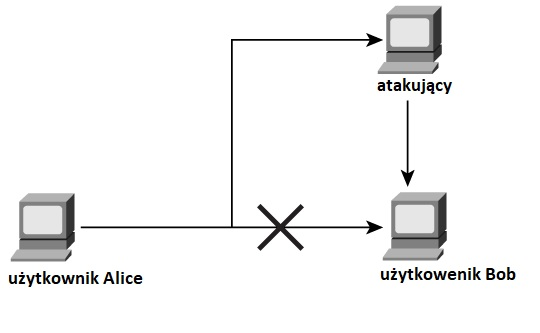
\includegraphics[width=7cm]{Powtarzajace_ataki.jpg}
\caption{Człowiek w środku - powtarzanie sesji}
\end{figure}

\quad W atakach typu "porwanie sesji" atakujący dodaje się do połączenia między dwoma użytkownikami w celu przejęcia komunikacji między nimi. Na rysunku poniżej pokazano schematycznie atak typu "porwanie sesji". Użytkownik Alice wysyła wiadomość do użytkownika Bob, jednak na drodze odczytuje ją atakujący, który przez Alice jest traktowany jako użytkownik Bob. Następnie atakujący przesyła wiadomość do prawdziwego Boba i po otrzymaniu jego odpowiedzi przesyła ją do użytkownika Alice po zmodyfikowaniu. Atakujący dołącza się do połączeń w celu znalezienie luk z zabezpieczeniach. Na rys. 1.2 przedstawiono schemat ataku typu człowiek w środku - porwanie sesji.
\begin{figure}[h]
\centering
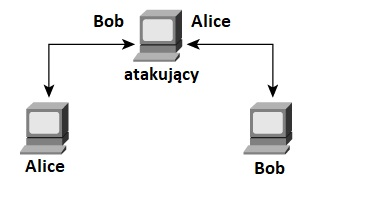
\includegraphics[width=8cm]{Porwanie_sesji.jpg}
\caption{Człowiek w środku - porwanie sesji}
\end{figure}

\quad Prywatna wirtualna sieć zapewnia trzy etapy chroniące nas przed niepożądanymi atakami w wystarczający sposób. Pierwszym z nich jest uwierzytelnienie urządzenia, które chroni przed przechwytywaniem pakietów przez zamaskowane urządzenia atakujące. Następnym krokiem jest sprawdzenie integralności pakietów np. przy użyciu funkcji haszujących. Trzecim etapem jest zaszyfrowanie pakietów, co znacznie utrudnia przechwycenie rzeczywistych informacji.
\end{itemize}


\subsection{Maszyna Enigma}

\subsection{Szyfry blokowe i strumieniowe}
\subsubsection{Szyfry blokowe} 
\quad Szyfry blokowe wykorzystywane są do szyfrowania i deszyfrowania. Danymi wejściowymi do szyfrowania jest blok danych, który przy użyciu klucza szyfrującego jest przekształcany w zaszyfrowany blok danych. Odszyfrowywanie przebiega w odwrotny sposób, zaszyfrowana blokowa wiadomość przy użyciu klucza jest transformowana do odszyfrowanej blokowej wiadomości. Szyfr blokowy jest bezpieczny do momentu kiedy klucz szyfrujący pozostaje tajny. Bez znajomości klucza niemożliwe staje się rozszyfrowanie wiadomości w satysfakcjonującym nas czasie. Im bardziej klucz jest przypadkowy tym ciężej złamać algorytm. Ważnymi parametrami szyfru blokowego jest rozmiar bloku i klucza od których to zależy bezpieczeństwo algorytmu. Powszechnie stosowanymi rozmiarami bloków są 64 i 128 bitowe bloki, zazwyczaj algorytm DES ma 64 bitowy blok danych, zaś AES 128 bitowy blok. 
\begin{figure}[h]
\centering
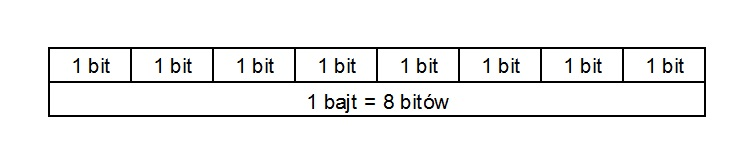
\includegraphics[width=12cm]{bajt.jpg}
\caption{Tu umieszczasz opis}
\end{figure}

\quad Długość zaszyfrowanego bloku musi być optymalna, im większe bloki danych tym dłuższy zaszyfrowany tekst oraz użycie pamięci. Przy szyfrowaniu wiadomości która na długość 8 bitową, zaś blok szyfru ma długość 64 bity najpierw 8 bitowa wiadomość zostanie prze konwertowana na 64 bitowy blok. Następnie 64 bitowa wiadomość zostanie zaszyfrowana przy użyciu algorytmu tworząc zaszyfrowany tekst. Do przetworzenia szyfru blokowego o rozmiarze 64 bitów potrzebujemy 64 bitów pamięci w rejestrach procesora. W dzisiejszych czasach procesory z pamięcią 64 bitową nie są kosztowne, lecz im większy chcemy utworzyć blok szyfrowy tym lepszy procesor potrzebujemy, co może mieć znaczny wpływ na wysokie koszty.

\subsubsection{Szyfry strumieniowe}

\subsection{Szyfry symetryczne i asymetryczne}

\subsubsection{Szyfry symetryczne}
\paragraph{DES}
\paragraph{AES}
\paragraph{IDEA}
\paragraph{Blowfish}
\subsubsection{Szyfry asymetryczne}
\paragraph{RSA}
\paragraph{Diffie-Hellman}
\paragraph{Funkcje haszujące}

\subsection{Protokoły}
\subsubsection{VPN with Point-to-Point Tunneling Protocol (PPTP)}
\quad Protokół punkt - punt często wykorzystywany na urządzeniach z systemem operacyjnym Windows w celu utworzenia wirtualnej sieci prywatnej. Protokół PPTP został utworzony w czasach sieci wdzwanianej tzn. dial up, jednak bez problemu można z niego korzystać również dla sieci Ethernet, Internet czy cyfrowa sieć usług zintegrowanych(ISDN). Utworzenie sicei VPN w sieci TCP/IP umożliwia bezpieczny transfer danych między zdalnym komputerem, a serwerem. Do implementacji protokołu głównie jest wykorzystywany: klient PPTP, serwer NAS i serwer PPTP. Serwer NAS bezpiecznie przechowuje dane i udostępnia je tylko wybranym użytkownikom. Na rys. 1.3 poniżej poglądowo przedstawiono komunikację z użyciem protokołu PPTP. 
\begin{figure}[h]
\centering
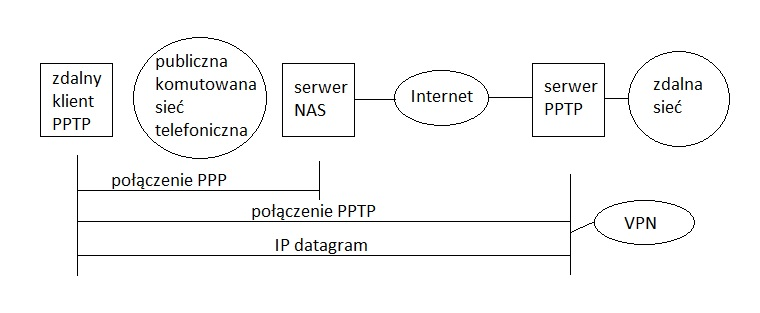
\includegraphics[width=12cm]{komunikacja_PPTP.jpg}
\caption{Poglądowa komunikacja z użyciem protokołu PPTP}
\end{figure}

Połączenie między zdalnym klientem, a siecią przebiega w określonych etapach:
\begin{itemize}
\item nawiązanie połączenia z użyciem protokołu komunikacyjnego point-to-point (PPP) między dwoma węzłami sieci w sposób telefoniczny bądź przewodowy z Internetem
\item połączenie PPP z serwerem PPTP, co tworzy połączenie VPN między zdalnym klientem, a serwerem
\end{itemize}
Po ustanowieniu połączenia wysyłane są dwa pakiety danych: pakiet kontrolny, który zarządza tunelem i pakiet danych. Protokół PPTP jest zaaplikowany na drugim poziomie modelu odniesienia łączenia systemów otwartych (OSI), który jest warstwą łącza danych. Jego działanie jest oparte na protokole punkt-punkt (PPP), który umożliwia korzystanie z usług internetowych. Protokół PPTP umożliwia firmom tworzenie prywatnych tuneli w publicznym internecie. Organizacje nie muszą już instalować kosztownych linii do komunikacji, dzięki protokołowi PPTP mogą w bezpieczny sposób korzystać z sieci publicznej w celu przesyłania poufnych danych. Protokół PPTP wspiera szyfrowanie i kompresję danych. Protokół PPTP nie jest wykorzystywany powszechnie ze względu na podatność na ataki.~\cite{PPTP}
\subsubsection{Secure Shell (SSH)}
\quad SSH z angielskiego to Secure Shell, co znaczy bezpieczna powłoka. Protokół SSH został wprowadzony w celu ulepszenia istniejących już wcześniej protokołów takich jak telnet, ftp czy BSD r-commands(rlogin, rexec, rsh,rcp). Protokoły telnet, ftp czy rsh były wykorzystywane do transferu plików między hostem lokalnym i zdalnym. Wymienione protokoły nadal są w powszechnym użytku, tylko tam gdzie bezpieczeństwo nie jest istotnym czynnikiem. Istotną wadą usług telnet i ftp jest brak szyfrowania i uwierzytelniania podczas przesyłania pakietów. Dane wysyłane są w sposób jawny, które mogą być w łatwiejszy sposób przechwycone przez atakującego. Atakujący może uzyskać niezaszyfrowane hasło, które następnie może wykorzystać w łatwy sposób. Wszędzie tam gdzie bezpieczeństwo danych jest ważne stosujemy protokół SSH. 
\quad SSH jest protokołem warstwy transportowej, która używa TCP do przenoszenia swoich pakietów. TCP jest protokołem sterowanie transmisją między dwoma urządzeniami. SSH umożliwia bezpieczne tunelowanie między lokalnym z zdalnym urządzeniem. Na poniższym rysunku przedstawiono komunikacje lokalnego klienta z powłoką serwera przy pomocy przekierowaniu portów. Na rys. 1.4 ukazano schemat lokalnego przekierowania portu dla protokołu SSH.
\begin{figure}[h]
\centering
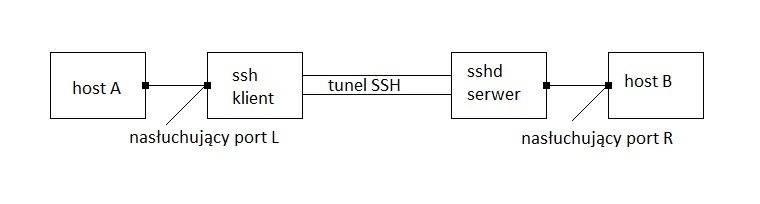
\includegraphics[width=12cm]{przekierowywanie_lokalne_SSH.jpg}
\caption{SSH lokalne przekierowywanie portu}
\end{figure}

Host A wykonuje bezpiecznie połączenie do hostu B poprzez port R. Połączenie hostu A z hostem B przebiega w następujący sposób:
\begin{itemize}
\item host A łączy się do porty L na kliencie SSH
\item SSH przekierowuje połączenie poprzez bezpieczny tunel do serwera SSH
\item serwer SSH łączy się z hostem B poprzez port R
\end{itemize}
\newpage Port L na hoście A i port R na hoście B ustawione są w trybie ciągłego nasłuchiwania dla lokalnego połączenia. Na rys. 1.5 przedstawiono zdalne przekierowywanie portu z hosta B do hosta.
 
\begin{figure}[h]
\centering
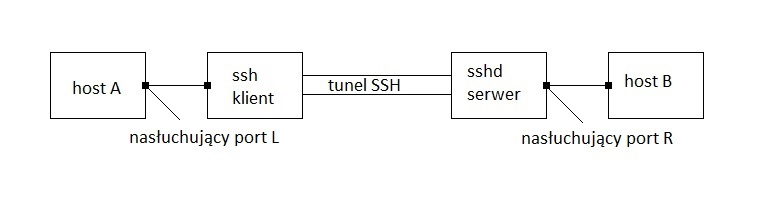
\includegraphics[width=10cm]{przekierowywanie_zdalne_SSH.jpg}
\caption{SSH zdalne przekierowywanie portu}
\end{figure}

Zdalne przekierowanie portu przebiega w następujących krokach:
\begin{itemize}
\item klient SSH wysyła żądanie zdalnego przekazywania portów, co powoduje nasłuchiwanie połączeń na porcie R po stronie serwera
\item przekiwrowanie połączenie przez bezpieczny tunel do klienta SSH
\item klient SSH łączy się do hosta A poprzez nasłuchujący port L po jego stronie
\end{itemize}
\quad 
Wykorzystując zjawisko tunelowania do prywatnej sieci wirtualnej tworzymy bezpieczne połączenie poprzez tunel między dwoma sieciami. ~\cite{SSH}

\subsubsection{IPsec}
\quad Protokół IPsec zawiera trzy główne protokoły:
\begin{itemize}
\item protokół uwierzytelnienie nagłówków (AH) - zapewnia uwierzytelnienie i integralność pakietów protokołu internetowego (IP)
\item  protokół bezpieczeństwa danych ESP - zapewnia te same usługi co protokół AH i dodatkowo zapewnia bezpieczeństwo danych
\item protokół wymiany klucza internetowego IKE - zapewnia zarządzanie kluczem, umożliwiając bezpiecznie skojarzenie dwóch hostów 
\end{itemize}
\quad Protokoły AH i ESP mogą działać w dwóch trybach: transportowym i tunelowym. Tryb transportowy zapewnia bezpieczeństwo dla warstw powyżej datagramu IP. Jest on inicjowany głównie między dwoma stałymi hostami, połączenie nie może być nawiązana między dwoma sieciami lub między siecią i hostem. Zaś tryb tunelowy zapewnia bezpieczeństwo całego datagramu IP. Jest on stosowany do połączenia tunelowego między dwoma sieciami lub między hostem, a siecią. Na rys. 1.6 poniżej przedstawiono schematyczny tryb tunelowy dla protokołu IPsec.
\begin{figure}[h]
\centering
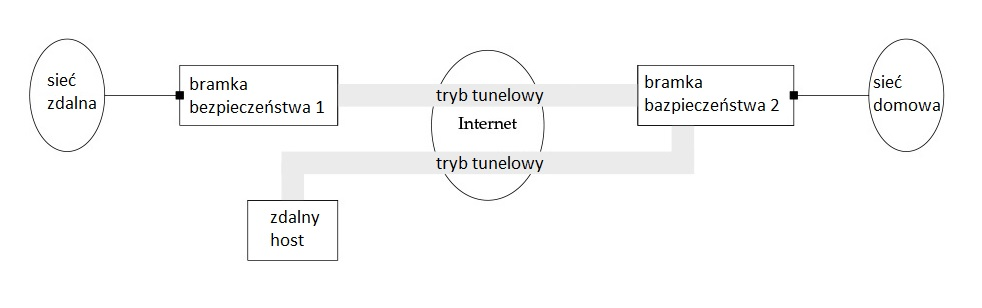
\includegraphics[width=10cm]{tryb_tunelowy_IPsec.jpg}
\caption{Tryb tunelowy IPsec}
\end{figure}
 
\quad Sieć zdalna jest połączona z siecią domową za pośrednictwem sieci tunelowej, bramki bezpieczeństwa 1 i bramki bezpieczeństwa 2. Funkcją bramek jest szyfrowanie, deszyfrowanie, zapobieganie ponownego odtwarzania wysyłanych pakietów i uwierzytelnianie. Z poziomu hostów bramki bezpieczeństwa i tunelowanie jest niewidoczne. Występują trzy metody uwierzytelnienie danych z udziałem protokołu bezpieczeństwa IPsec: wstępnie uzgodnione klucze, klucze prywatne i publiczne RSA oraz certyfikaty. Nagłówki uwierzytelniające dla trybu transportowego i tunelowego różnią się od siebie. Powszechny pakiet IP wchodzący w wyższą warstwę TCP składa się z: nagłówka IP, nagłówka TCP i danych użytkownika. Dla trybu transportowego nagłówek uwierzytelnienia dla IPsec składa się z: nagłówka IP, nagłówka uwierzytelniającego, nagłówka TCP i danych użytkownika. W tunelowym trybie nagłówek uwierzytelniający kopiuje część wewnętrzną nagłówka IP, która jest używana do utworzenia nowego zewnętrznego nagłówka IP. Nagłówek składa się z: zewnętrznego nagłówka IP, nagłówka uwierzytelniającego, wewnętrznego nagłówka IP, nagłówka TCP i danych użytkownika.

IPsec korzysta z protokołu Internet Key Exchange (IKE) w celu nawiązania i ustanowienie bezpiecznego połączenia między dwoma hostami lub zdalnego dostępu tunelowania VPN. Protokół IKE występuje w dwóch wersjach IKEv1 i IKEv2. Protokół IKEv1 można podzielić na dwie fazy, pierwsza w nich odpowiada za następujące funkcjonalności: algorytmy szyfrowania, algorytmy haszowania, protokół Diffiego-Hellmana oraz metodę uwierzytelniania.  Faza druga IKEv1 jest głównie używana do szyfrowania w protokole IPsec. Do szyfrowania wykorzystujemy algorytmy Data Encryption Standard (DES),  Triple DESo długości 168 bitów czy Advanced Encryption Standard (AES) o długości 128-256 bitów. Spośród wymienionych powyżej algorytmów DES zapewnia najniższe bezpieczeństwo danych, zaś AES o długości klucza 256 bitów największe bezpieczeństwo. Algorytmy haszujące zastosowane w protokole IPsec to: Secure Hash Algorithm (SHA) oraz Message Digest 5 (MD5). Protokół MD5 jest mniej bezpieczny niż algorytm SHA.
Kiedy używamy IPsec wraz z VPN przesyłane dane będą zabezpieczone podczas przesyłania, w celu uniemożliwienia atakującemu zdobycie jawnych danych.  Proces szyfrowania, który zapewnia poufność przesyłanych danych nie daje możliwości łatwej modyfikacji wrażliwych danych atakującemu.

 Do stworzenia protokołu IPsec zrzeszenia bezpieczeństwa(Security Association AS) używanych jest kilka komponentów, które służą do przetwarzania ruchu tekstu jawnego, który jest chroniony i następnie przekształcany w tekst zaszyfrowany. Te same komponenty są używane do odszyfrowania danych. Protokół IPsec korzysta z trzech baz danych: 
\begin{itemize}
\item Baza danych zasad zabezpieczeń - Security Policy Database (SPD) określa jaki ruch ma być chroniony
\item Baza danych stowarzyszenia zabezpieczeń - Security Association Database (SAD) określa w jaki sposób ruch jest chroniony
\item Baza danych autoryzacji - Peer Authorization Database (PAD) zapewnia mechanizm wymuszający  politykę z oparciu o protokół IKE
\end{itemize}

\subsubsection{Secure Socket Tunneling protocol Based on VPN}
\quad Protokół SSTP umożliwia administratorom na ustanowienie tunelów poprzez główną sieć korporacyjną na Windows Serwer. Dzięki zredukowanie wymaganych kroków technicznych do utworzenia tunelów między organizacjami zyskujemy niższy koszt administracyjny. Brak dodatkowych zmian w infrastrukturze dla protokołu SSTP, gdyż podobnie jak w protokóle HTTPS jest obsługiwana zapora sieciowa i serwery proxy. Protokół SSTP wykorzystuje protokołu SSL do transportu ruchu sieciowego. SSL jest certyfikatem odpowiedzialnym za poświadczenie wiarygodności domeny bądź jej właściciela, co zapewnia bezpieczeństw szyfrowania danych. PPP to protokół połączenie punkt-punkt. Protokołem odpowiedzialnym za sterowanie transmisją jest TCP. 
Proces utworzenia połączenia wykorzystującego VPN między klientem, a serwerem przebiega w następujący sposób:
\begin{itemize}
\item klient ustanawia połączenie TCP z serwerem SSTP pomiędzy dynamicznie zaalokowanym portem TCP po stronie klienta SSTP, a portem TCP 443 na serwerze SSTP
\item klient SSTP wysyła wiadomość Witaj SSL świadczącą o chęci nawiązania połączenia SSL z serwerem SSTP
\item serwer SSTP wysyła do klienta cyfrowy certyfikat
\item klient SSTP sprawdza poprawność certyfikatu, wybiera metodę szyfrowania dla sesji SSL, generuje klucze i następnie szyfruje certyfikat serwera przy użyciu klucza publicznego
\item klient SSTP wysyła zaszyfrowany klucz sesji SSL do serwera SSTP
\item serwer SSTP odszyfrowuje zaszyfrowany klucz sesji SSL z wykorzystaniem klucza prywatnego; dalsza komunikacja klienta z serwerem jest zaszyfrowana wybraną metodą szyfrowania i odszyfrowywana kluczem sesji SSL
\item klient wysyła komunikat HTTP poprzez sesję SSL do serwera
\item klient ustala połączenie tunelowe z serwerem
\item klient SSTP ustala połączenie PPP z serwerem SSTP, które obejmuje uwierzytelnienie danych logowanie użytkownika wraz z uwierzytelnieniem PPP i ustawieniem konfiguracji ruchu IP
\item klient SSTP rozpoczyna proces ruchu sieciowego IP poprzez łącze PPP~\cite{SSTP}
\end{itemize}

\subsubsection{L2TP}
\quad Protokół tunelujący warstwy 2 (Layer 2 Tunneling Protocol L2TP) działa na warstwie łączy danych, która jest drugą w siedmio warstwowym modelu odniesienia łączenia systemów otwartych (OSI). Protokół ten nie zapewnia szyfrowania ani poufności danych, z tego powodu jest często używany z protokołem IPsec który zapewnia szyfrowanie i poufność danych. Protokół służy do komunikacji między klientem zwanym jako koncentrator dostępu L2TP(LAC) oraz serwerem nazywanym sieciowym serwerem L2TP (LNS). 
Protokół L2TP, który jest wykorzystywany do włączenie sieci VPN w Internecie jest rozszerzeniem protokołu PPTP. Powstał on w połączeniu protokołu firmy PPTP opracowanej przez Microsoft i L2F (przekierowywanie warstwy drugiej modelu OSI) firmy Cisco. Połączenie użytkownika domowego do sieci firmowej wykorzystujące protokół L2TP i połączenie internetowe przedstawiono w następujących krokach:
\begin{itemize}
\item zdalny użytkownik korzysta z analogowego połączenia telefonicznego lub łącza szerokopasmowego w celu zainicjowania połączenie PPP do dostawcy usług internetowych
\item sieć LAC akceptuje połączenie co prowadzi do ustanowienia połączenia PPP
\item w czasie gdy użytkownik końcowy i serwer nawiązują połączenie, koncentrator dostępu LAC rozpoczyna uwierzytelniania użytkownika metodą CHAP lub PAP
\item po pomyślnie ukończonym procesie uwierzytelnienia, połączenie użytkownika z serwerem LNS zostaje pomyślnie nawiązane; w przypadku niepomyślnego procesu uwierzytelnienie klient uzyskuje dostęp do Internetu jako normalny użytkownik
\item punkty końcowe tunelu (LAC i LNS) przed wysłaniem danych poprzez tunel uwierzytelniają się wzajemnie
\item po utworzeniu tunelu VPN korzystającego z protokołu L2TP połączenie między użytkownikiem, a siecią korporacyjną zostaje nawiązane 
\end{itemize}
Protokół L2TP jest protokołem sieci komputerowej wykorzystywanym przez dostawców internetowych do utworzenia wirtualnej sieci prywatnej między dwoma urządzeniami.~\cite{L2TP}

\newpage
\section{Systemy wbudowane}
\subsection{Budowa }
\paragraph{Rejestr} % rejestr i rejsster specjalny
\paragraph{Pamięć} % nieulotne i ulotne
\paragraph{Porty wejścia/wyjścia}
\paragraph{Centralne jednostka obliczeniowa}
\paragraph{Dekoder instrukcji}
\paragraph{Jednostka arytmetyczno-logiczna ALU}
\paragraph{Rejestr SREG}
\paragraph{Zegar}
\paragraph{Magistrala}
\paragraph{Linie danych, adresowe i sterowania}

\subsection{Architektura systemów wbudowanych}
\quad Architekturę systemów wbudowanych możemy podzielić na architekturę zależną od struktury pamięci i zależną od typu instrukcji. Struktura pamięci : harwardzka, zmodyfikowana harwardzka i von-Neumanna. Typu instrukcji RISC i CISC.
\subsubsection{Architektura harwardzka}
\subsubsection{Zmodyfikowana architektura harwardzka}
\subsubsection{Architektura von-Neumanna}
\subsubsection{RISC - Recuded Instruction Set Computer}
\subsubsection{CISC - Complex Instruction Set Computer}

\newpage
\section{Aplikacja algorytmów kryptograficznych na systemie wbudowanym}
  ...
\subsection{Charakterystyka systemu wbudowanego}
\subsection{Implementacja algorytmów szyfrujących}
\subsubsection{Implementacja szyfru Cezara}
\subsubsection{Implementacja szyfru AES}
\subsection{Wyniki implementacji algorytmów szyfrujących} 
\newpage
\section{Wnioski}
\section{Podsumowanie}

\newpage
\begin{thebibliography}{99}

\bibitem{PPTP} D. Stoddard i T.M. Thomas,
\emph{
Cover image for Network Security First-Step, Second Edition
Network Security First-Step, Second Edition},
Cisco Press, 12.2011, chapter 6

\bibitem{SSH} A. Lockhart,
\emph{Network Security Hacks},
O'Reilly Media Inc., 04.2004, chapter 6

\bibitem{SSTP} J. Savill,
\emph{The Complete Guide to Windows Server 2008},
Addison-Wesley Professional, 10.2008, chapter 8

\bibitem{L2TP} S. Malik,
\emph{Cover image for Network Security Principles and Practices
Network Security Principles and Practices},
Cisco Press, 10.2002

\end{thebibliography}
\newpage
\listoffigures
\addcontentsline{toc}{section}{Literatura}
\addcontentsline{toc}{section}{Spis rysunków}

\end{document}
